\chapter{Magnetic field induced by harmonic current in a wire}

\modinfo{Directory}{MagneticFieldWire}
\modinfo{Solvers}{\Idx{WhitneyAVHarmonicSolver}}
\modinfo{Tools}{\Idx{ElmerGrid}, \Idx{ElmerGUI}}
\modinfo{Dimensions}{3D, Harmonic}
\modinfo{Author}{Peter R{\aa}back}


\subsection*{Case definition}

This case demonstrates the simplest case on how to utilize the edge element based solvers
for computation of magnetic and electric fields.

Consider a simple copper wire with radius $R=0.001$~m and length $R=0.01$~m. A potential difference of 1~V/m is applied
over the wire. We want to know the magnetic field strength around the wire.  

For steady state we have a simple analytical solution for reference.
\begin{equation}
\vec{A} = \left \{
\begin{array}{ll}
  -\frac{I\mu_0}{2\pi}\ln (r/R) \vec{e}_z, & \, \, \, r > R \\
  -\frac{I\mu_0}{4\pi R^2 } (r^2 - R^2) \vec{e}_z, & \, \, \, r \leq R 
\end{array}  
\right .
\end{equation}
resulting to a magnetic flux density
\begin{equation}
\vec{B} = \left \{
\begin{array}{ll}
  \frac{I\mu_0}{2\pi r}\vec{e}_\phi, & \, \, \, r > R \\
  \frac{I\mu_0}{2\pi R}\frac{r}{R}\vec{e}_\phi, & \, \, \, r \leq R 
\end{array}  
\right .
\end{equation}
We can solve the current from Ohms law to obtain the maximum field value at $r=R$ to be
\begin{equation}
  | \vec{B} | = \frac{1}{2} \mu_0 R \sigma | \vec{E} |   
\end{equation}
Using electric conductivity of copper ($\sigma$=59.59e6 A/m$^2$V) we obtain 0.0374~T.

We are interested in what happens when the voltage is applied sinusoidally with a frequency of 100~kHz.
The harmonic case is unfortunately much more difficult to solve and no simple analytical expression exists.
Therefore we need to solve the problem numerically. 


\subsection*{Solution procedure}

This tutorial will need the additional EDF, \texttt{\Idx{magnetodynamics.xml}}, for the WhitneyAVHarmonic Solver.  The definitions for the relevant equation are not loaded into ElmerGUI by default. Hence, 
one needs to load these before starting the simulations.
\ttbegin
File 
  Definitions
    Append -> magnetodynamics.xml
\ttend
The additional definitions should reside in the directory \texttt{edf-extra} within the distribution.
Moving the desired \texttt{xml} files to the \texttt{edf}-directory enables automatic loading of the 
definitions at start-up. By inspecting the definitions in the \texttt{Elmer Definitions File editor} one
may inspect that the new definitions were really appended. 

The mesh is already defined in ElmerGrid format as file \texttt{wire.grd}. Load it from the tutorial directory where it resides.
\ttbegin
File 
  Open -> wire.grd
\ttend
The ElmerGrid plug-in of ElmerGUI will read the mesh and create the mesh for ElmerGUI using the ElmerGrid plug-in.
Note that the user
could also create the mesh directly on the command line by
\ttbegin
ElmerGrid 1 2 wire.grd
\ttend
and then use the \texttt{Load Mesh} option in \texttt{ElmerGUI} to take the mesh into use. 
If the user wants to modify the default mesh that can be done by editing the file directly.
The mesh has been constructed so that it can capture some boundary layer phenomena that we expect to take
place on the surface of the wire. In principle the mesh could be even shorter since the results do not really
depend on the axial direction. 


\begin{figure}[h]
\centering
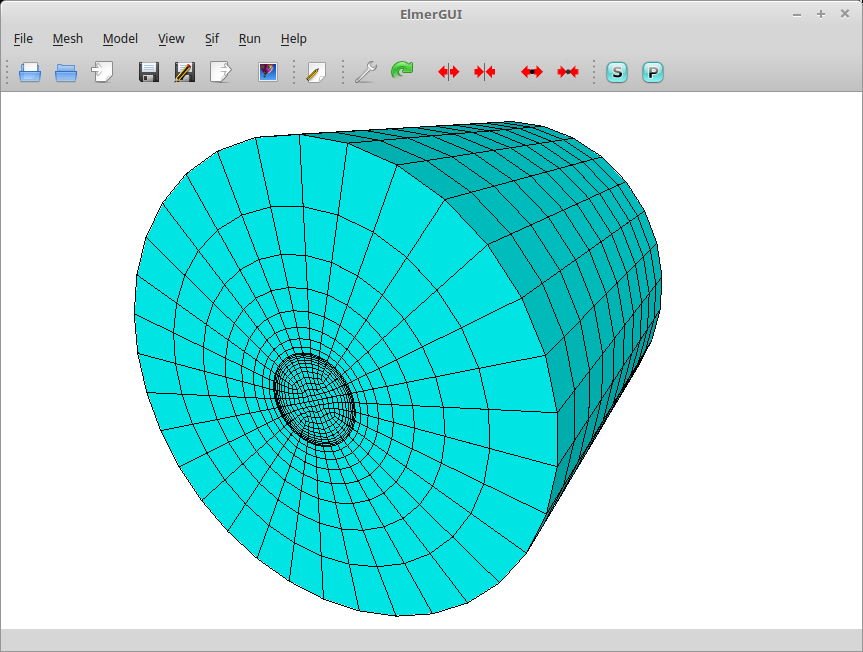
\includegraphics[width=140mm]{WireElmerGUI}
\caption{The mesh for the wire and surrounding air as seen in ElmerGUI}\label{fg:WireElmerGUI}
\end{figure}  


After we have the mesh we start to go through the Model menu from the top to bottom.

In the Setup we choose things related to the whole simulation such as file names, 
time stepping, constants etc.
The steady-state simulation is carried out in 3-dimensional Cartesian
coordinates. The initial size of the mesh is in millimeters, which is 1000 times too large. Hence we apply scaling in this menu, Coordinate Scaling = 1.0e-3.  Enter a single scaling number, and the scaling will be applied equally to all coordinates, whether in 2D or 3D.

Also we want to use a harmonic equation that requires the frequency to be set somewhere, in this case we will define the frequency in the Simulation section. 
\ttbegin
SetUp
  Coordinate Scaling 
    1.0e-3
  Angular Frequency
    1.0e5   
\ttend
The permeability of vacuum is predefined in SI Units in the Constants section. To set other than the default value for it (in case using a different unit system),
change the value in the Constants section.

In the equation section we choose the relevant equations and parameters related to their solution. 
In this case we'll have the \texttt{\Idx{MgHarm}} solver (there exists also a steady-state/transient version of the solver
as \texttt{\Idx{MgDyn}}), as well as the postprocessing solver \texttt{\Idx{MgDynPost}}.

When defining Equations and Materials it is possible to assign to the bodies immediately, or to use mouse
selection to assign them later. In this case we know that body 1 is the wire and body 2 is the surrounding air and we
can apply the definitions directly.
They will have the same set of solvers but different material properties. 

The solver specific options may need some alternations. We choose a more suitable
linear solver strategy for the AV equation. 

For the postprocessing we add some fields to be computed and skip the computation of nodal fields since the
elemental fields are often preferable for discontinuous fields. 
We also want to ensure that the postprocessing solver is run just before saving the results, after the primary solver has been computed.

In the following the correct equation are chosen and the suitable solver specific options are chosen:
\ttbegin
Model
  Equation
    Name = MgHarm
      Active = on
      Apply to Bodies = 1 2  
      Edit Solver Settings
        Linear System
          Iterative = BiCGStabL
        Preconditioning = none
        BiCGStabl order = 4    
    Name = MgDynPost
      Active = on
      Edit Solver Settings
        Solver Specific Options
          Calculate Magnetic Field Strength = on
          Calculate Joule Heating = on
          Skip Nodal Field = on
          Discontinuous Bodies = on
        General
          Execute Solver = before saving   
    Add 
    OK
\ttend        
The Material section includes all the material parameters. In this case we basically have two 
different materials -- the copper wire and the surrounding air.
We use the definitions from the small material database that comes with the code, and the material properties are in SI Units.
\ttbegin
Model
  Material
    Material Library
      Copper
    Apply to Bodies = 1
    Add
    New

  Material
    Material Library
      Air (room temperature)
    Apply to Bodies = 2
    Add
    OK
\ttend

We need to set the boundary conditions both for the scalar potential associated to the nodal degrees of freedom, \texttt{av},
and to the vector potential associated to the edge degrees of freedom, \texttt{av \{e\}}.
Both of these have both real and imaginary components. 
We set the scalar potential only for the conductors and the vector potential for all external boundaries.
\ttbegin
Model
  BoundaryCondition
    Name = Ground 
    MgHarm
      AV re = 0
      AV re {e} 1 = 0
      AV re {e} 2 = 0
      AV im = 0
      AV im {e} 1 = 0
      AV im {e} 2 = 0
    Add
    OK
\ttend   
For the other of the wire we have exactly the same BCs except that the scalar potential is set to 0.01~V to give the desired
electric field of 1~V/m, since the length of the wire is 0.01~m. 
\ttbegin
Model
  BoundaryCondition
    Name = Voltage
    MgHarm
      AV re = 0.01
      AV re {e} 1 = 0
      AV re {e} 2 = 0
      AV im = 0
      AV im {e} 1 = 0
      AV im {e} 2 = 0
    Add
    OK
\ttend   
and finally for all other external BCs we set the boundary non-axial components of the vector potential to zero.
\ttbegin
Model
  BoundaryCondition
    Name = AxialField
    MgHarm
      AV re {e} 1 = 0
      AV re {e} 2 = 0
      AV im {e} 1 = 0
      AV im {e} 2 = 0
    Add
    OK
\ttend 


The conditions may also be assigned to boundaries in the Boundary condition menu, or 
by clicking with the mouse. Here we use the latter approach as that spares us of the 
need to know the indexes of each boundary.
\ttbegin
Model
  Set boundary properties
    Choose one end of the wire -> set boundary condition to Ground
    Choose the other end of the wire -> set boundary condition to Voltage
    Choose all other external BCs -> set boundary condition to AxialField
\ttend

For the execution 
ElmerSolver needs the mesh files and the command file. We have now basically defined
all the information for ElmerGUI to write the command file. After writing it we may also visually 
inspect the command file.
\ttbegin
Sif 
  Generate
  Edit -> look how your command file came out  
\ttend

Before we can execute the solver we should save the files in a directory. The project includes
all the files needed to restart the case.
\ttbegin
File 
  Save Project
\ttend

After we have successfully saved the files we may start the solver
\ttbegin
Run
  Start solver
\ttend
A convergence view automatically pops up showing relative changes of each iteration.
The equation is fully linear and hence only two iterations are needed -- the second 
one just ensures that convergence of the non-linear level was really obtained. 
The convergence monitor also plots the postprocessing steps but they do not really converge as each field is computed just once. 

When the solution has finished we may start the postprocessor to view some results.
\ttbegin
Run
  Start ParaView
\ttend


\subsection*{Results}

Here we present some results of the computations. The visualization is done using Paraview and the \texttt{vtu} format.
For optimal visualization turn on the \texttt{\Idx{Discontinuous Bodies}} flag on both on the calculation of the fields
and while saving the results in \texttt{vtu} format. 
These flags ensure that the solution is continuous within the bodies while maintaining jumps between bodies. 
No other formats in Elmer can currently support these features.

The resulting absolute values of the imaginary and real part of the magnetic flux density are depicted in
Figure~\ref{fg:BfieldWire-im} and Figure~\ref{fg:BfieldWire-re}. The imaginary part dominates in the amplitude (im 0.00522~T vs. re 0.00111~T). 
The corresponding vector field of the magnetic flux density is depicted in Figure~\ref{fg:BfieldWireVectors}.

Why are the results so far from the steady state solution? If you run the case again with 
100~Hz you can see that the solution is very close to the static one as shown in Figure~\ref{fg:BfieldWire-re-100}. The maximum magnetic flux density from the 
computations is 0.0366~T which is very close to the analytical solution of 0.0374~T. So the frequency
really has an significant effect on the results!

You may study what happens when you increase the frequency further. At some point the mesh cannot capture the solution
properly any more and the results become questionable.

\begin{figure}[H]
\centering
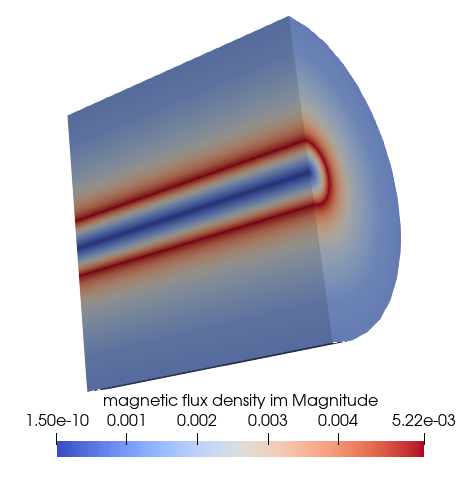
\includegraphics[width=0.6\textwidth]{mag-flux-dens-im-100k}
\caption{Imaginary part of the magnetic flux density at 100k Hz.}
\label{fg:BfieldWire-im}
\end{figure}  

\begin{figure}[H]
\centering
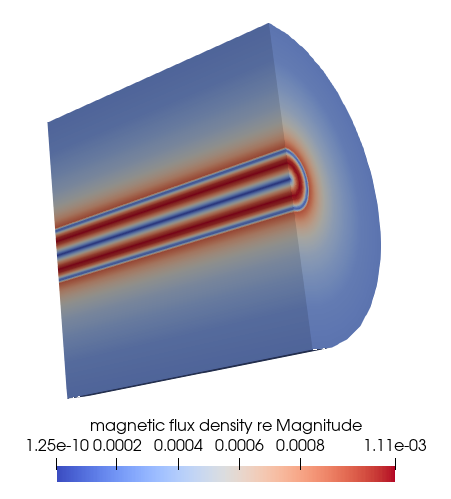
\includegraphics[width=0.6\textwidth]{mag-flux-dens-re-100k}
\caption{Real part of the magnetic flux density at 100k Hz.}
\label{fg:BfieldWire-re}
\end{figure}  

\begin{figure}[H]
\centering
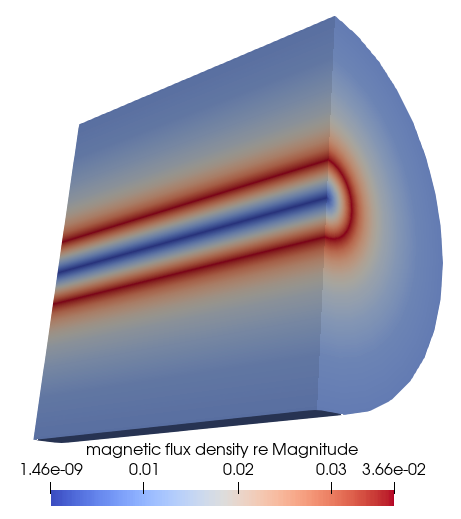
\includegraphics[width=0.6\textwidth]{mag-flux-dens-re-100}
\caption{Real part of the magnetic flux density at 100 Hz.}
\label{fg:BfieldWire-re-100}
\end{figure}  

\begin{figure}[H]
\centering
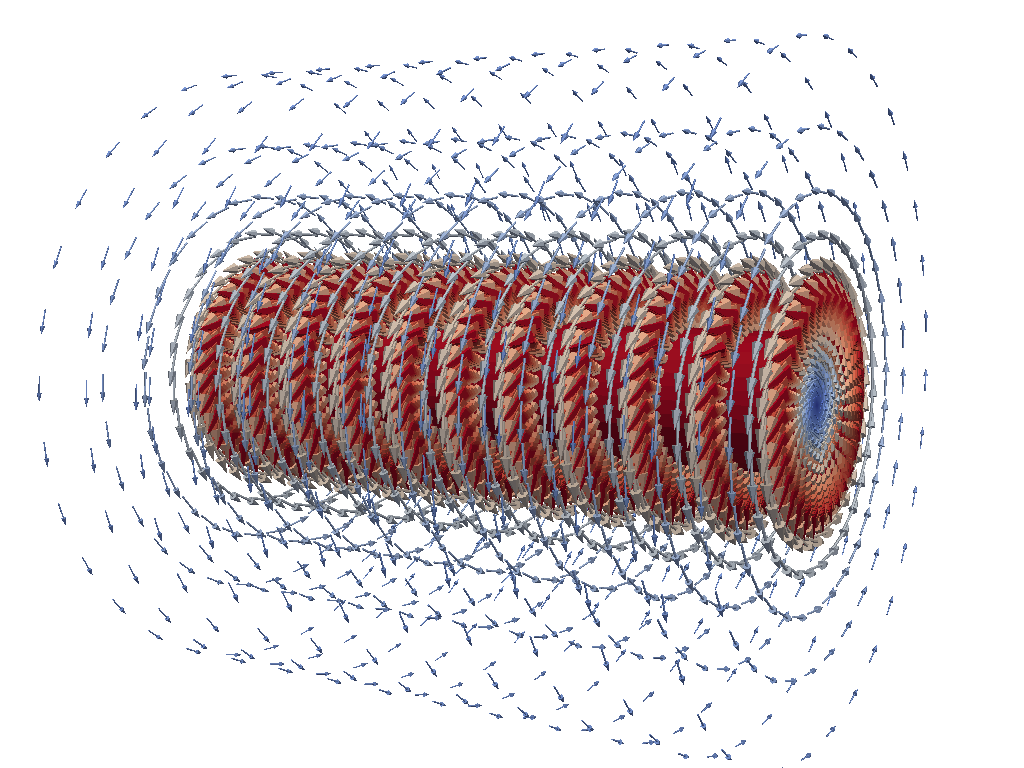
\includegraphics[width=0.7\textwidth]{WireBfieldImVectors}
\caption{Imaginary part of the magnetic field strength plotted with vectors scaled by the field values.}
\label{fg:BfieldWireVectors}
\end{figure}  

